\documentclass[aspectratio=169,professionalfonts]{beamer}

\usetheme{crystalite}

\usepackage{amsmath}
\usepackage{amssymb}
\usepackage{booktabs}
\usepackage{graphicx}
\usepackage{pgfplots}
\usepackage{siunitx}
\usepackage{tabularx}
\usepackage{array}
\usepackage{bm}
\usepackage{hyperref}

\graphicspath{{assets/images/}}
\pgfplotsset{compat=1.18}
\sisetup{detect-all}
\hypersetup{colorlinks=true,urlcolor=crystaliteaccentdark,linkcolor=crystaliteaccentdark}

\title{Crystalite Presentation Preset}
\subtitle{A Beamer starter translated from the Crystalite blogpost into an editorial slide format with bundled fonts, figure cards, and restrained scientific plotting styles.}
\crystalitekicker{Mar 2026 / Research Presentation}
\author{Tin Hadzi Veljkovic}
\institute{Materials ML / Diffusion Models}
\date{Compile with \texttt{latexmk main.tex}}

\begin{document}

\begin{frame}[plain]
  \titlepage
\end{frame}

\section{Style System}

\begin{frame}{Design Translation}{What the preset keeps from the article}
  \small
  \begin{columns}[T,onlytextwidth]
    \column{0.56\textwidth}
    \begin{itemize}
      \item Soft blue-white paper background instead of flat white.
      \item Dark slate typography with quiet metadata labels.
      \item Rounded white figure cards rather than heavy boxes.
      \item Blue-lilac accents reserved for dividers and plots.
    \end{itemize}
    \column{0.4\textwidth}
    \begin{crystalitenote}
      \crystalitemeta{Practical note}

      The article itself mixes web fonts. This preset bundles local files so the deck can live
      offline.
    \end{crystalitenote}
    \vspace{0.2cm}

    {\color{crystalitemuted}\scriptsize Best suited to research talks, paper explainers, and thesis
    updates that need a calmer editorial tone than stock Beamer.}
  \end{columns}
\end{frame}

\begin{frame}{Typography And Components}{Reusable ingredients included in the preset}
  \small
  \begin{columns}[T,onlytextwidth]
    \column{0.48\textwidth}
    \begin{block}{Body copy}
      Keep paragraph text brief, then move dense detail into cards, tables, or figure captions.
    \end{block}

    \vspace{0.18cm}

    \begin{alertblock}{Callout}
      Pair one key equation or chart with one short note instead of stacking multiple equally heavy
      elements.
    \end{alertblock}
    \column{0.48\textwidth}
    \begin{crystalitepanel}
      \crystalitemeta{Equation example}

      \vspace{0.15cm}
      \[
        \mathcal{C} = (\mathbf{H}, \mathbf{F}, \mathbf{y}),
        \qquad
        \mathbf{y} \in \mathbb{R}^{6}.
      \]
    \end{crystalitepanel}

    \vspace{0.18cm}

    {\ttfamily\scriptsize\color{crystalitemuted}
    Metadata, code, and commands use the same mono voice.}
  \end{columns}
\end{frame}

\section{Figures}

\begin{frame}{Fractional Coordinates}{Image-first layout with editorial captioning}
  \small
  \begin{columns}[T,onlytextwidth]
    \column{0.62\textwidth}
    \begin{crystalitepanel}
      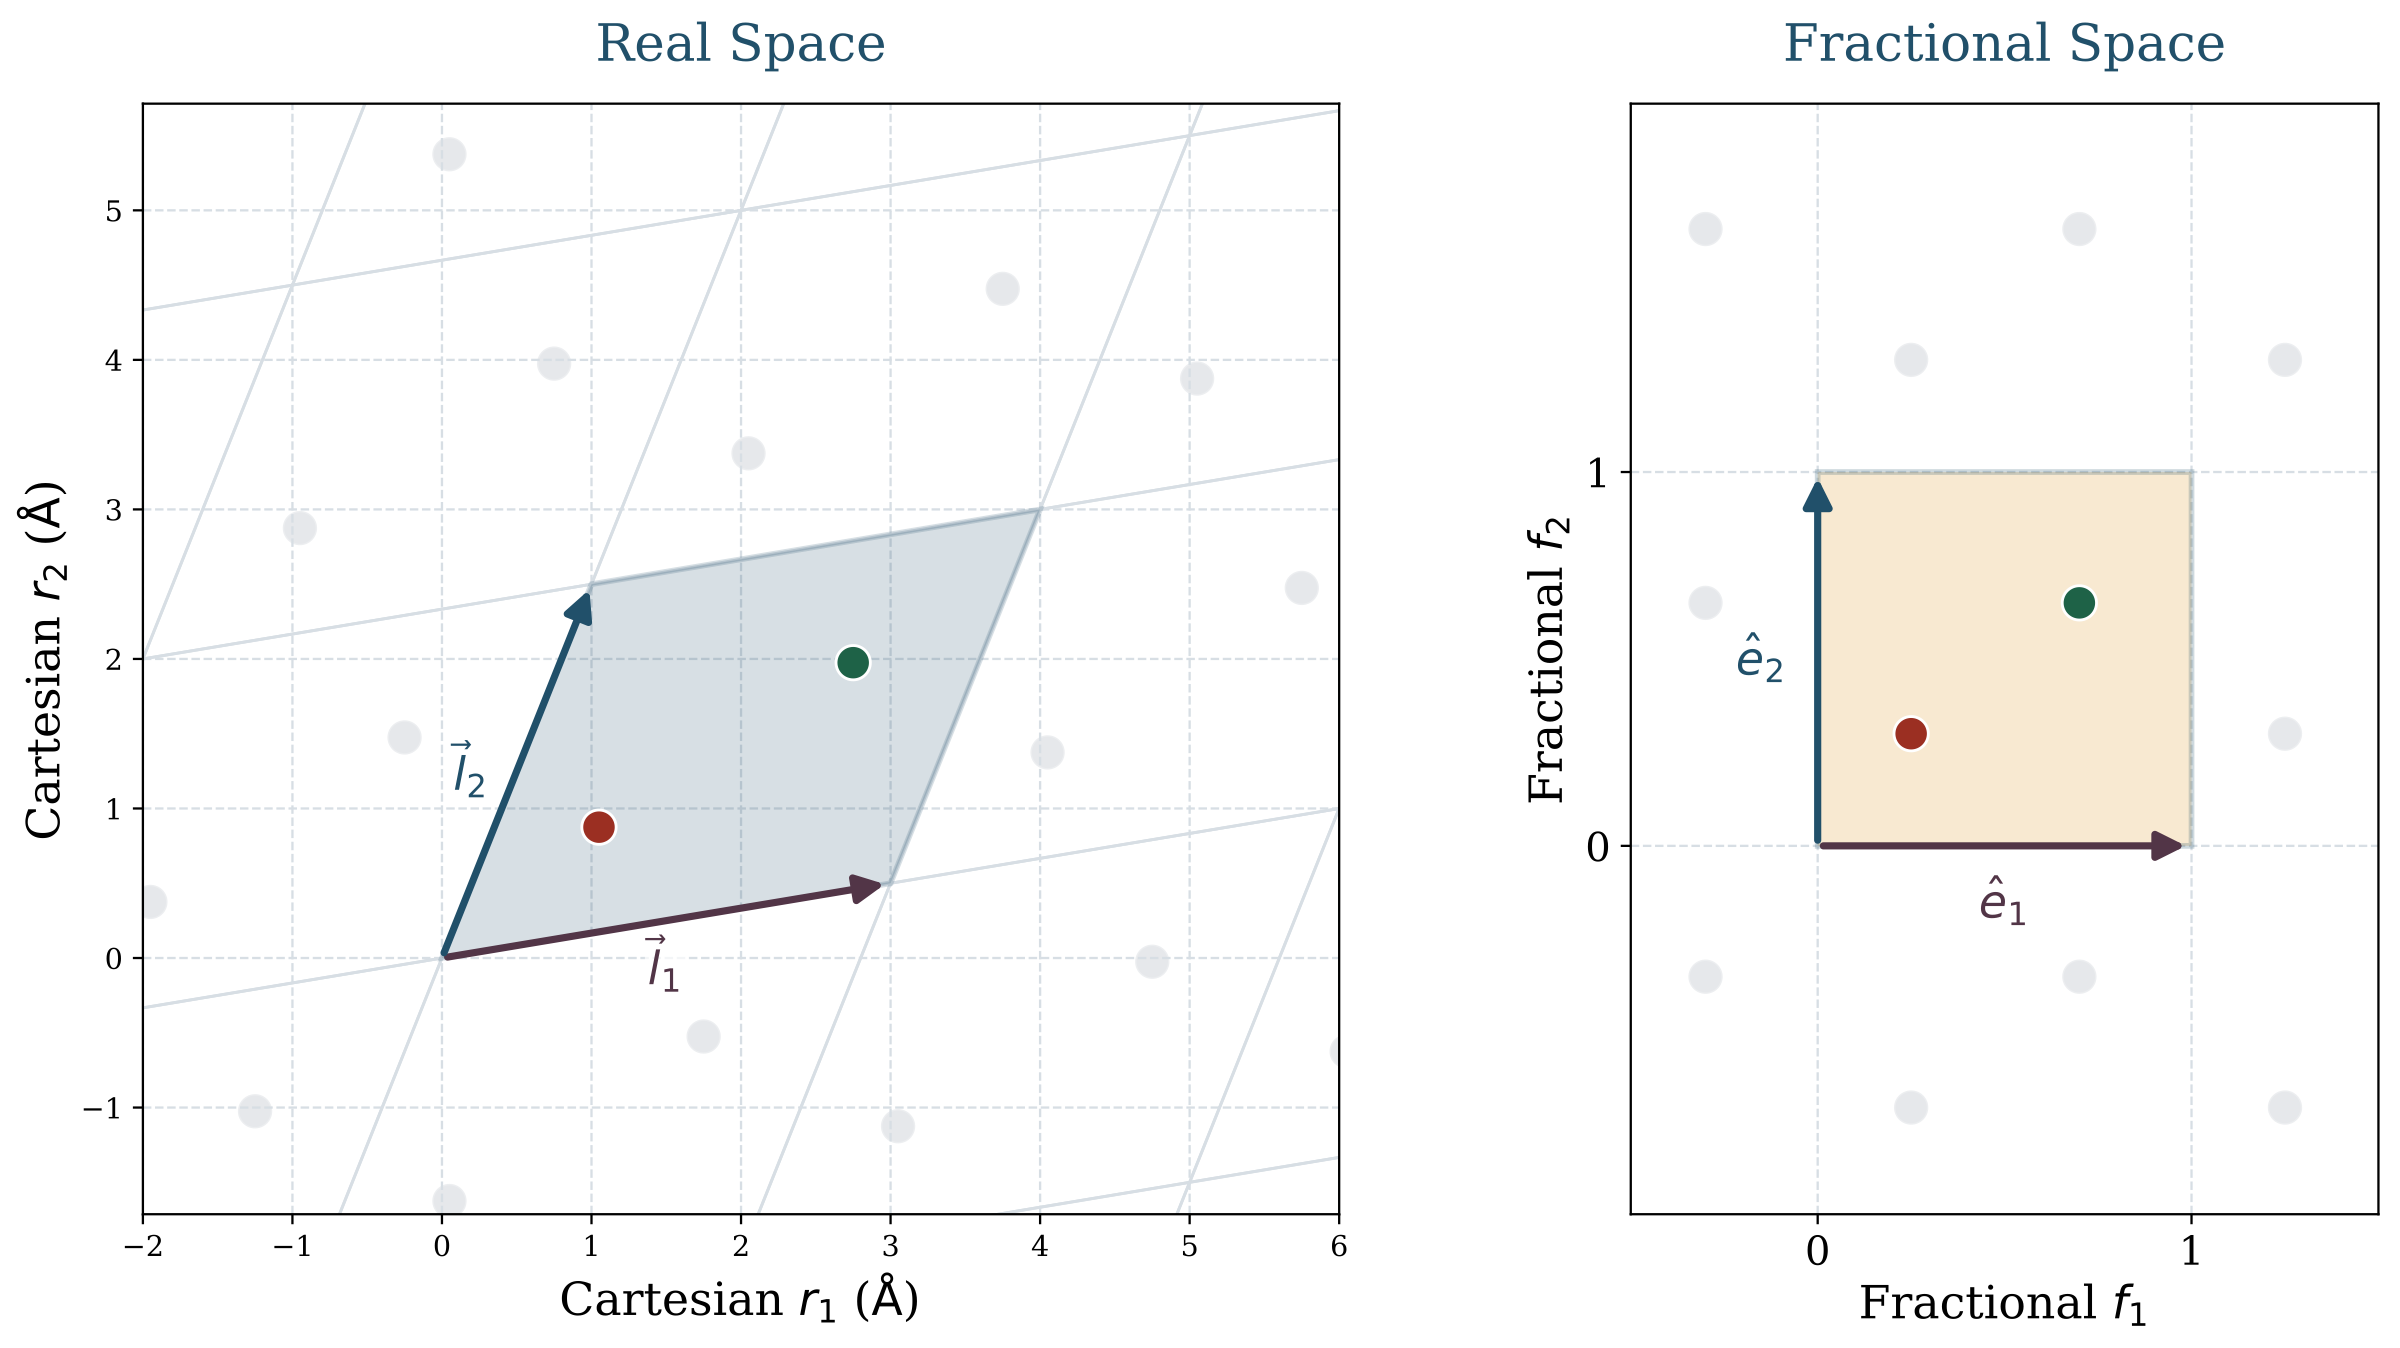
\includegraphics[width=\linewidth,height=3.8cm,keepaspectratio]{frac-coords.png}
      \crystalitecaption{Rounded panel framing mirrors the article's figure treatment.}
    \end{crystalitepanel}
    \column{0.34\textwidth}
    \begin{itemize}
      \item Use one dominant figure per slide.
      \item Keep labels off the image when possible.
      \item Let the caption carry context.
    \end{itemize}
  \end{columns}
\end{frame}

\begin{frame}{Architecture Slide Pattern}{Pair a system diagram with one decisive takeaway}
  \small
  \begin{columns}[T,onlytextwidth]
    \column{0.58\textwidth}
    \begin{crystalitepanel}
      
\includegraphics[width=\linewidth,height=3.95cm,keepaspectratio]{crystalite-architecture.png}
      \crystalitecaption{Use architecture diagrams inside white cards, then trim the prose around
      them.}
    \end{crystalitepanel}
    \column{0.38\textwidth}
    \begin{block}{Message hierarchy}
      One token per atom, one global lattice token, and periodic geometry injected through
      attention rather than a heavy fully equivariant trunk.
    \end{block}
    \vspace{0.2cm}

    {\color{crystalitemuted}\scriptsize Use the right column for the spoken thesis. The figure
    shows how; the text says why.}
  \end{columns}
\end{frame}

\begin{frame}{Method Detail}{Compact equation plus supporting figure}
  \small
  \begin{columns}[T,onlytextwidth]
    \column{0.42\textwidth}
    \begin{crystalitepanel}
      \crystalitemeta{Periodic-image search}

      \vspace{0.2cm}
      \[
        \Delta \mathbf{f}_{ij}^{\star}
        =
        \arg\min_{\mathbf{r} \in \Omega_R}
        \left\|
        \left( \mathbf{f}_i - \mathbf{f}_j + \mathbf{r} \right)\mathbf{L}
        \right\|_2.
      \]

      \vspace{0.2cm}

      Dense notation can sit next to a visual without flattening the hierarchy.
    \end{crystalitepanel}
    \column{0.54\textwidth}
    \begin{crystalitepanel}
      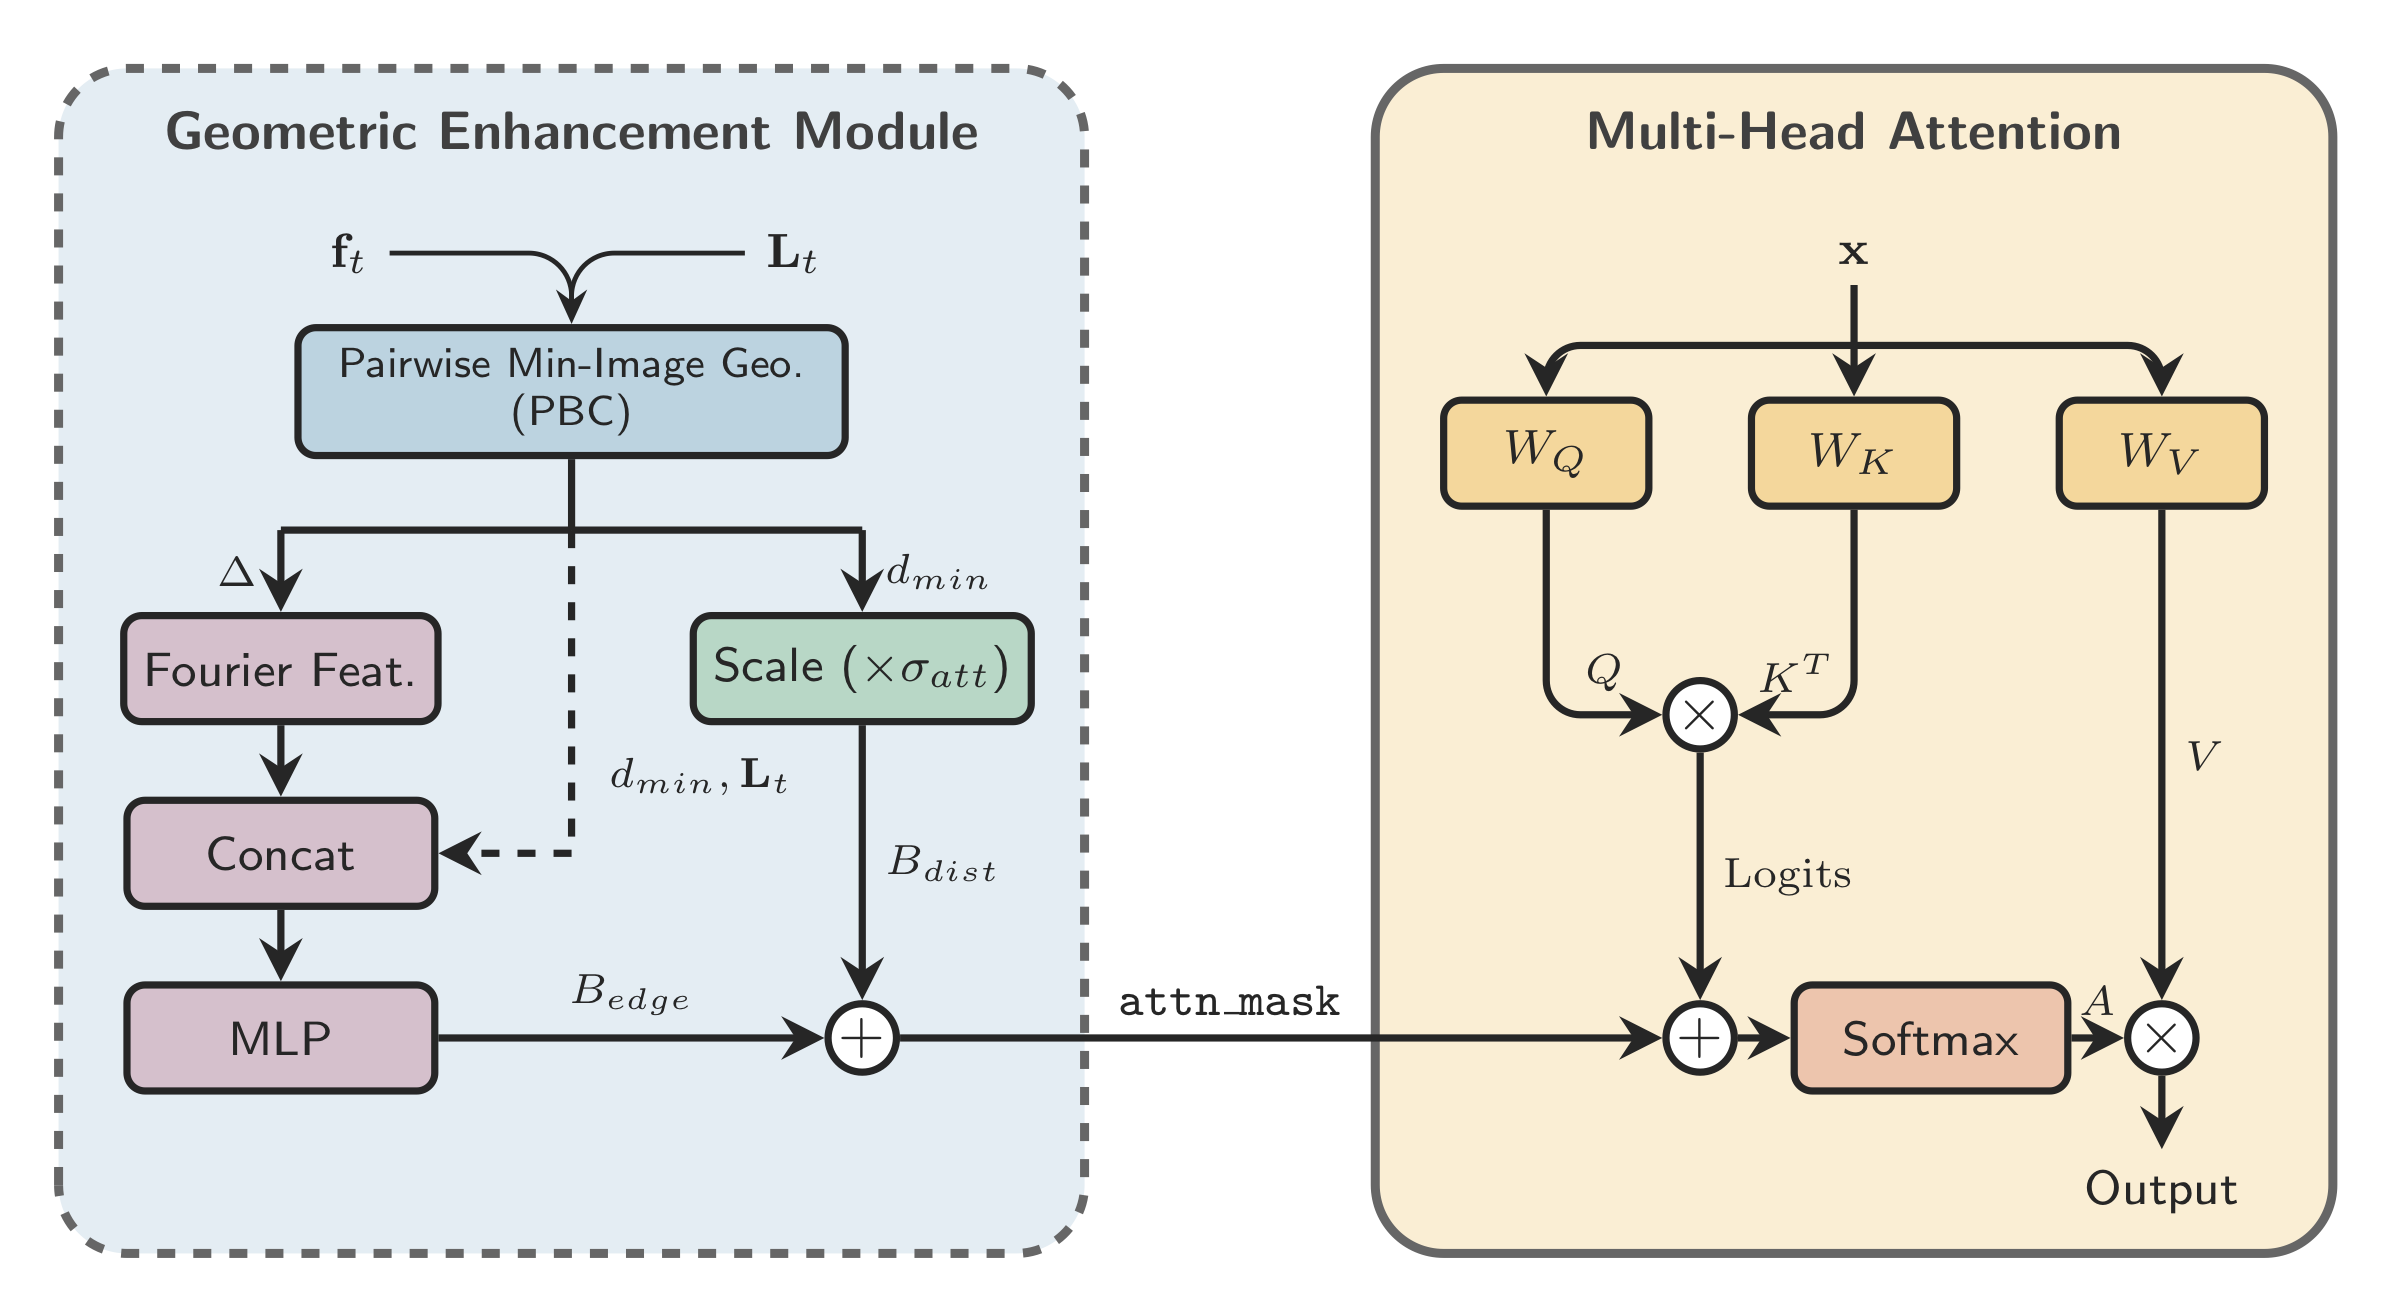
\includegraphics[width=\linewidth,height=4.2cm,keepaspectratio]{gem-module.png}
      \crystalitecaption{A second figure card works well for a method submodule or ablation
      visual.}
    \end{crystalitepanel}
  \end{columns}
\end{frame}

\section{Results}

\begin{frame}{Example Plot Styles}{Two editable plot templates are included}
  \small
  \begin{columns}[T,onlytextwidth]
    \column{0.5\textwidth}
    \begin{crystalitepanel}
      \crystalitemeta{Illustrative scaling curve}

      \begin{tikzpicture}
        \begin{axis}[
          width=\linewidth,
          height=4.35cm,
          xmin=250,
          xmax=10250,
          ymin=0.48,
          ymax=0.96,
          axis line style={draw=crystaliteline},
          tick style={draw=crystaliteline},
          tick label style={font=\scriptsize, text=crystalitemuted},
          label style={font=\scriptsize, text=crystalitemuted},
          grid=major,
          grid style={draw=crystaliteline},
          xlabel={sampling budget},
          ylabel={score},
          legend style={
            draw=none,
            fill=none,
            font=\scriptsize,
            text=crystaliteink,
            at={(0.03,0.97)},
            anchor=north west
          }
        ]
          \addplot[
            smooth,
            very thick,
            color=crystaliteaccentdark
          ] table[x=budget,y=crystalite,col sep=comma] {data/sample_efficiency.csv};
          \addlegendentry{light backbone}

          \addplot[
            smooth,
            very thick,
            color=crystaliteaccentb!75!crystaliteaccentdark
          ] table[x=budget,y=baseline,col sep=comma] {data/sample_efficiency.csv};
          \addlegendentry{heavier baseline}
        \end{axis}
      \end{tikzpicture}
    \end{crystalitepanel}
    \column{0.46\textwidth}
    \begin{crystalitepanel}
      \crystalitemeta{Illustrative runtime chart}

      \begin{tikzpicture}
        \begin{axis}[
          width=\linewidth,
          height=4.35cm,
          ybar,
          bar width=11pt,
          ymin=0,
          ymax=3.8,
          symbolic x coords={Crystalite,Hybrid,EquivariantGNN,HeavyDiffusion},
          xtick=data,
          axis line style={draw=crystaliteline},
          tick style={draw=crystaliteline},
          tick label style={font=\scriptsize, text=crystalitemuted, rotate=18, anchor=east},
          yticklabel style={font=\scriptsize, text=crystalitemuted},
          ylabel={relative runtime},
          label style={font=\scriptsize, text=crystalitemuted},
          nodes near coords,
          every node near coord/.append style={font=\scriptsize, text=crystaliteink},
          enlarge x limits=0.15
        ]
          \addplot[
            fill=crystaliteaccenta!85!white,
            draw=crystaliteaccentdark
          ] table[x=model,y=runtime,col sep=comma] {data/runtime_tradeoff.csv};
        \end{axis}
      \end{tikzpicture}
    \end{crystalitepanel}
  \end{columns}

  {\color{crystalitemuted}\scriptsize Editable CSV placeholders are bundled for both plots.}
\end{frame}

\begin{frame}{Image-Driven Results Slide}{Large visual plus compact benchmark summary}
  \small
  \begin{columns}[T,onlytextwidth]
    \column{0.6\textwidth}
    \begin{crystalitepanel}
      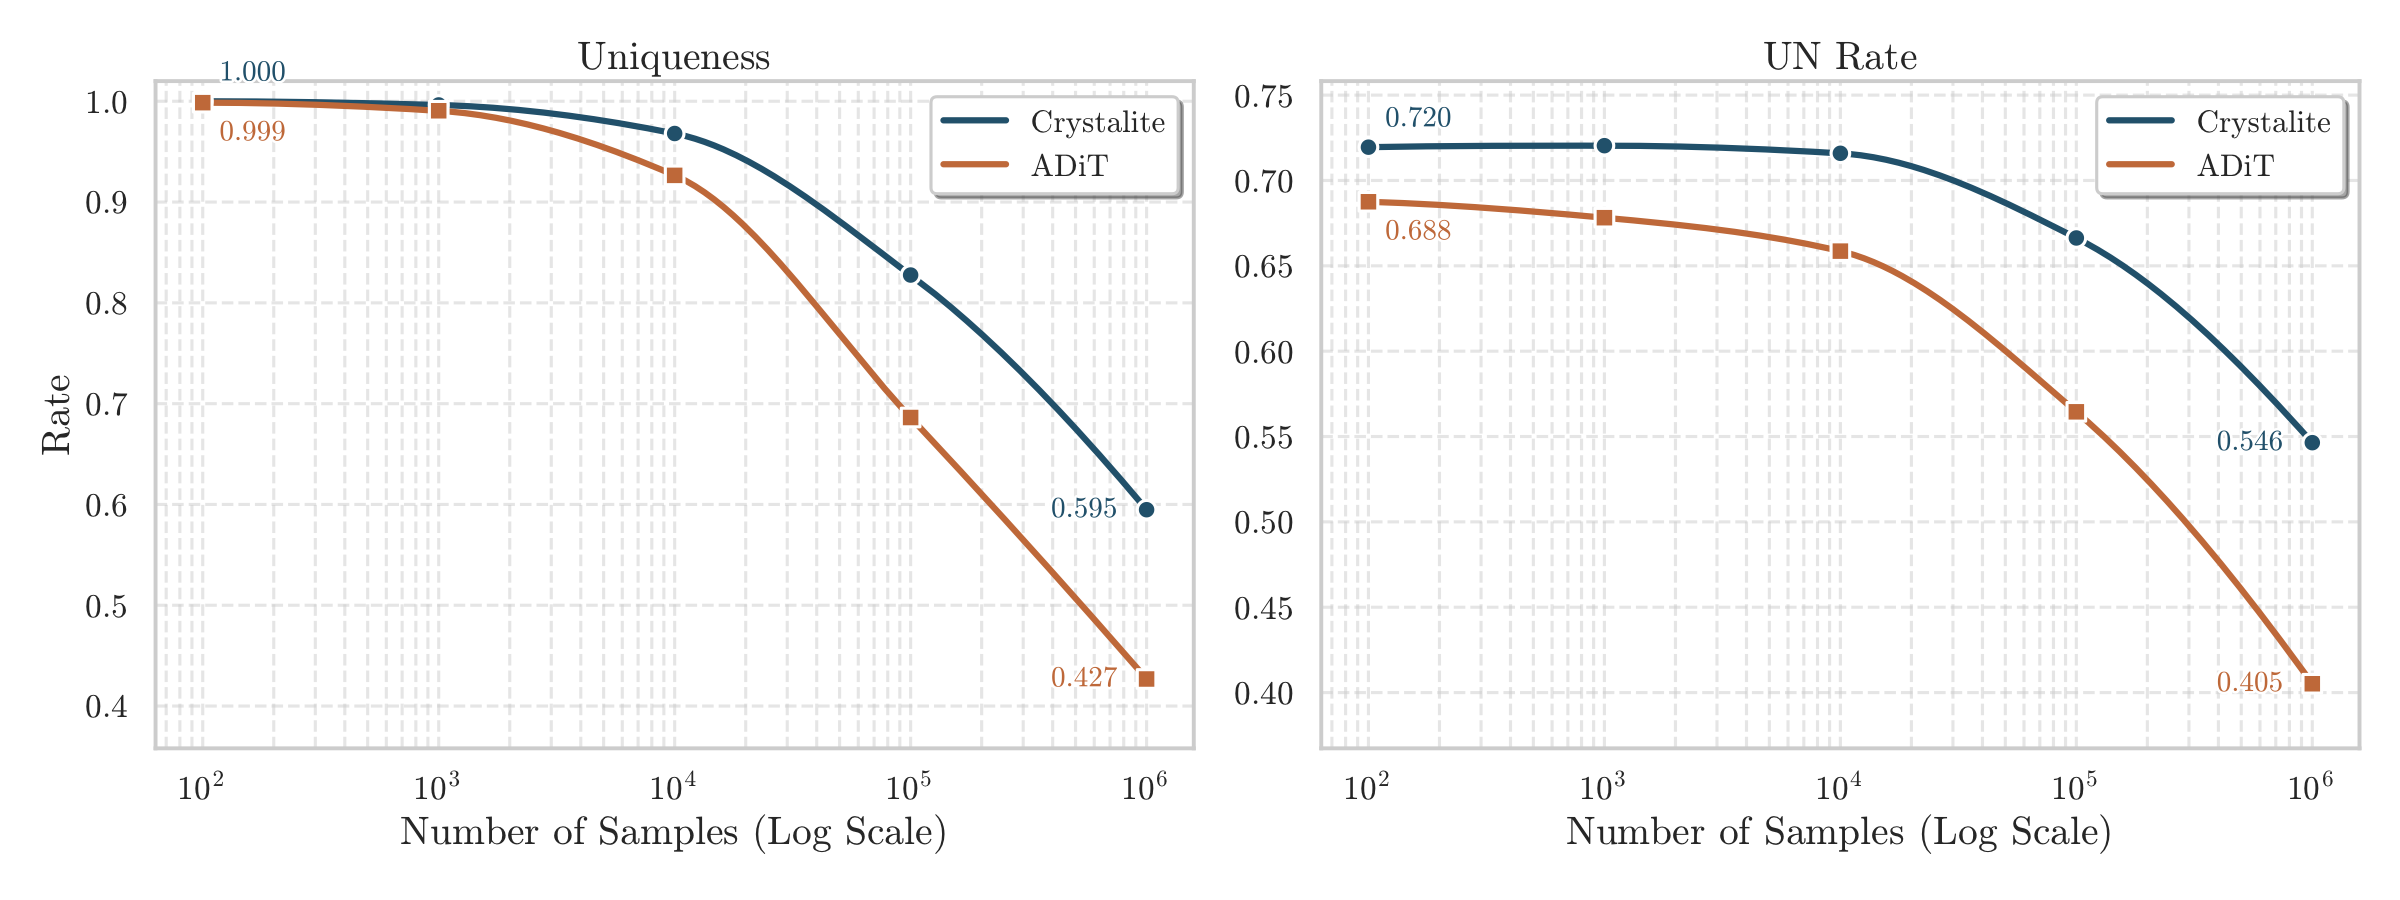
\includegraphics[width=\linewidth,height=4.0cm,keepaspectratio]{large-scale-generation.png}
      \crystalitecaption{This pattern works well for benchmark overviews or qualitative generation
      galleries.}
    \end{crystalitepanel}
    \column{0.36\textwidth}
    \begin{crystalitepanel}
      \crystalitemeta{Benchmark snapshot}

      \small
      \begin{tabularx}{\linewidth}{@{}>{\bfseries}l>{\raggedleft\arraybackslash}X@{}}
        \toprule
        Metric & Value \\
        \midrule
        Match rate & 0.83 \\
        RMSE & 0.049 \\
        S.U.N. & 0.79 \\
        Relative runtime & 1.00 \\
        \bottomrule
      \end{tabularx}
    \end{crystalitepanel}
    \vspace{0.18cm}

    {\color{crystalitemuted}\scriptsize Keep tables short and move the full benchmark to the
    appendix.}
  \end{columns}
\end{frame}

\section{Template Use}

\begin{frame}{Starting A New Deck}{Minimal source skeleton}
\scriptsize
\begin{crystalitepanel}
\ttfamily
\detokenize{\documentclass[aspectratio=169]{beamer}}\par
\detokenize{\usetheme{crystalite}}\par
\detokenize{\title{Your Talk Title}}\par
\detokenize{\crystalitekicker{Apr 2026 / Conference Talk}}\par
\detokenize{\author{Your Name}}\par
\par
\detokenize{\begin{document}}\par
\detokenize{\begin{frame}[plain]}\par
\hspace*{1em}\detokenize{\titlepage}\par
\detokenize{\end{frame}}\par
\detokenize{\section{Problem}}\par
\detokenize{\begin{frame}{One strong slide title}}\par
\hspace*{1em}\detokenize{Your content here.}\par
\detokenize{\end{frame}}\par
\detokenize{\end{document}}\par
\end{crystalitepanel}
\end{frame}

\begin{frame}{Included Files}{What is bundled in this folder}
  \small
  \begin{itemize}
    \item \texttt{beamerthemecrystalite.sty}: theme, colors, typography, cards, and section slides.
    \item \texttt{main.tex}: example deck with text, equations, figures, tables, and plots.
    \item \texttt{assets/fonts/}: copied local fonts so the deck builds offline.
    \item \texttt{assets/images/}: copied Crystalite figures for immediate reuse.
    \item \texttt{data/*.csv}: placeholder benchmark data for the plot templates.
    \item \texttt{Makefile} and \texttt{latexmkrc}: one-command build helpers.
  \end{itemize}

  \vspace{0.3cm}

  \begin{crystalitenote}
    If you want a darker inverse variant later, it is straightforward to add a second palette on
    top of the same layout and typography system.
  \end{crystalitenote}
\end{frame}

\begin{frame}[plain]
  \vspace*{1cm}
  {\color{crystalitemuted}\crystalitemeta{Closing slide}\par}
  \vfill
  {\usebeamerfont{title}Crystalite makes a good presentation language because it is restrained,
  legible, and visual without becoming ornamental.\par}
  \vspace{0.45cm}
  {\color{crystalitemuted}\fontsize{12}{16}\selectfont
    Replace the example content, keep the spacing discipline, and the deck will stay coherent.\par}
  \vfill
  {\ttfamily\small\color{crystalitemuted}presentations/crystalite-beamer}
\end{frame}

\end{document}
